\subsection{Scelte di Design} \label{sec:design-choices}
In questa sezione le scelte architetturali vengono analizzate in dettaglio, 
specificando come ci aspettiamo che il sistema verrà organizzato da un punto di vista
implementativo. Grazie a dei diagrammi UML l'applicazione prende forma negli aspetti più
tecnici che verranno poi rispettati nella fase di implementazione.

\subsubsection{Casi d'uso} \label{sec:design-choices:use-cases}
I casi d'uso espongono l'applicazione da un punto di vista strettamente funzionale,
specificando le azioni che l'utente può compiere durante le varie fasi del gioco.

In figura \ref{fig:use-cases} sono riportati i casi d'uso dell'applicazione Scala Party.
Sono suddivisi nelle schermate principali del gioco:
\begin{itemize}
    \item \textbf{Start Screen}: è la schermata iniziale del gioco, in cui l'utente
    può scegliere di iniziare una nuova partita o di visualizzare le regole del gioco.
    \item \textbf{Party Game}: è la schermata principale del gioco, in cui il giocatore
    può lanciare i dadi, muovere il proprio personaggio e ottenere gli oggetti collezionabili.
    \item \textbf{Minigame}: è la schermata in cui viene mostrato il minigioco
    attivo, in cui l'utente può visualizzare le regole e interagire con il minigioco.
\end{itemize}

\begin{figure}[ht!]
    \centering
    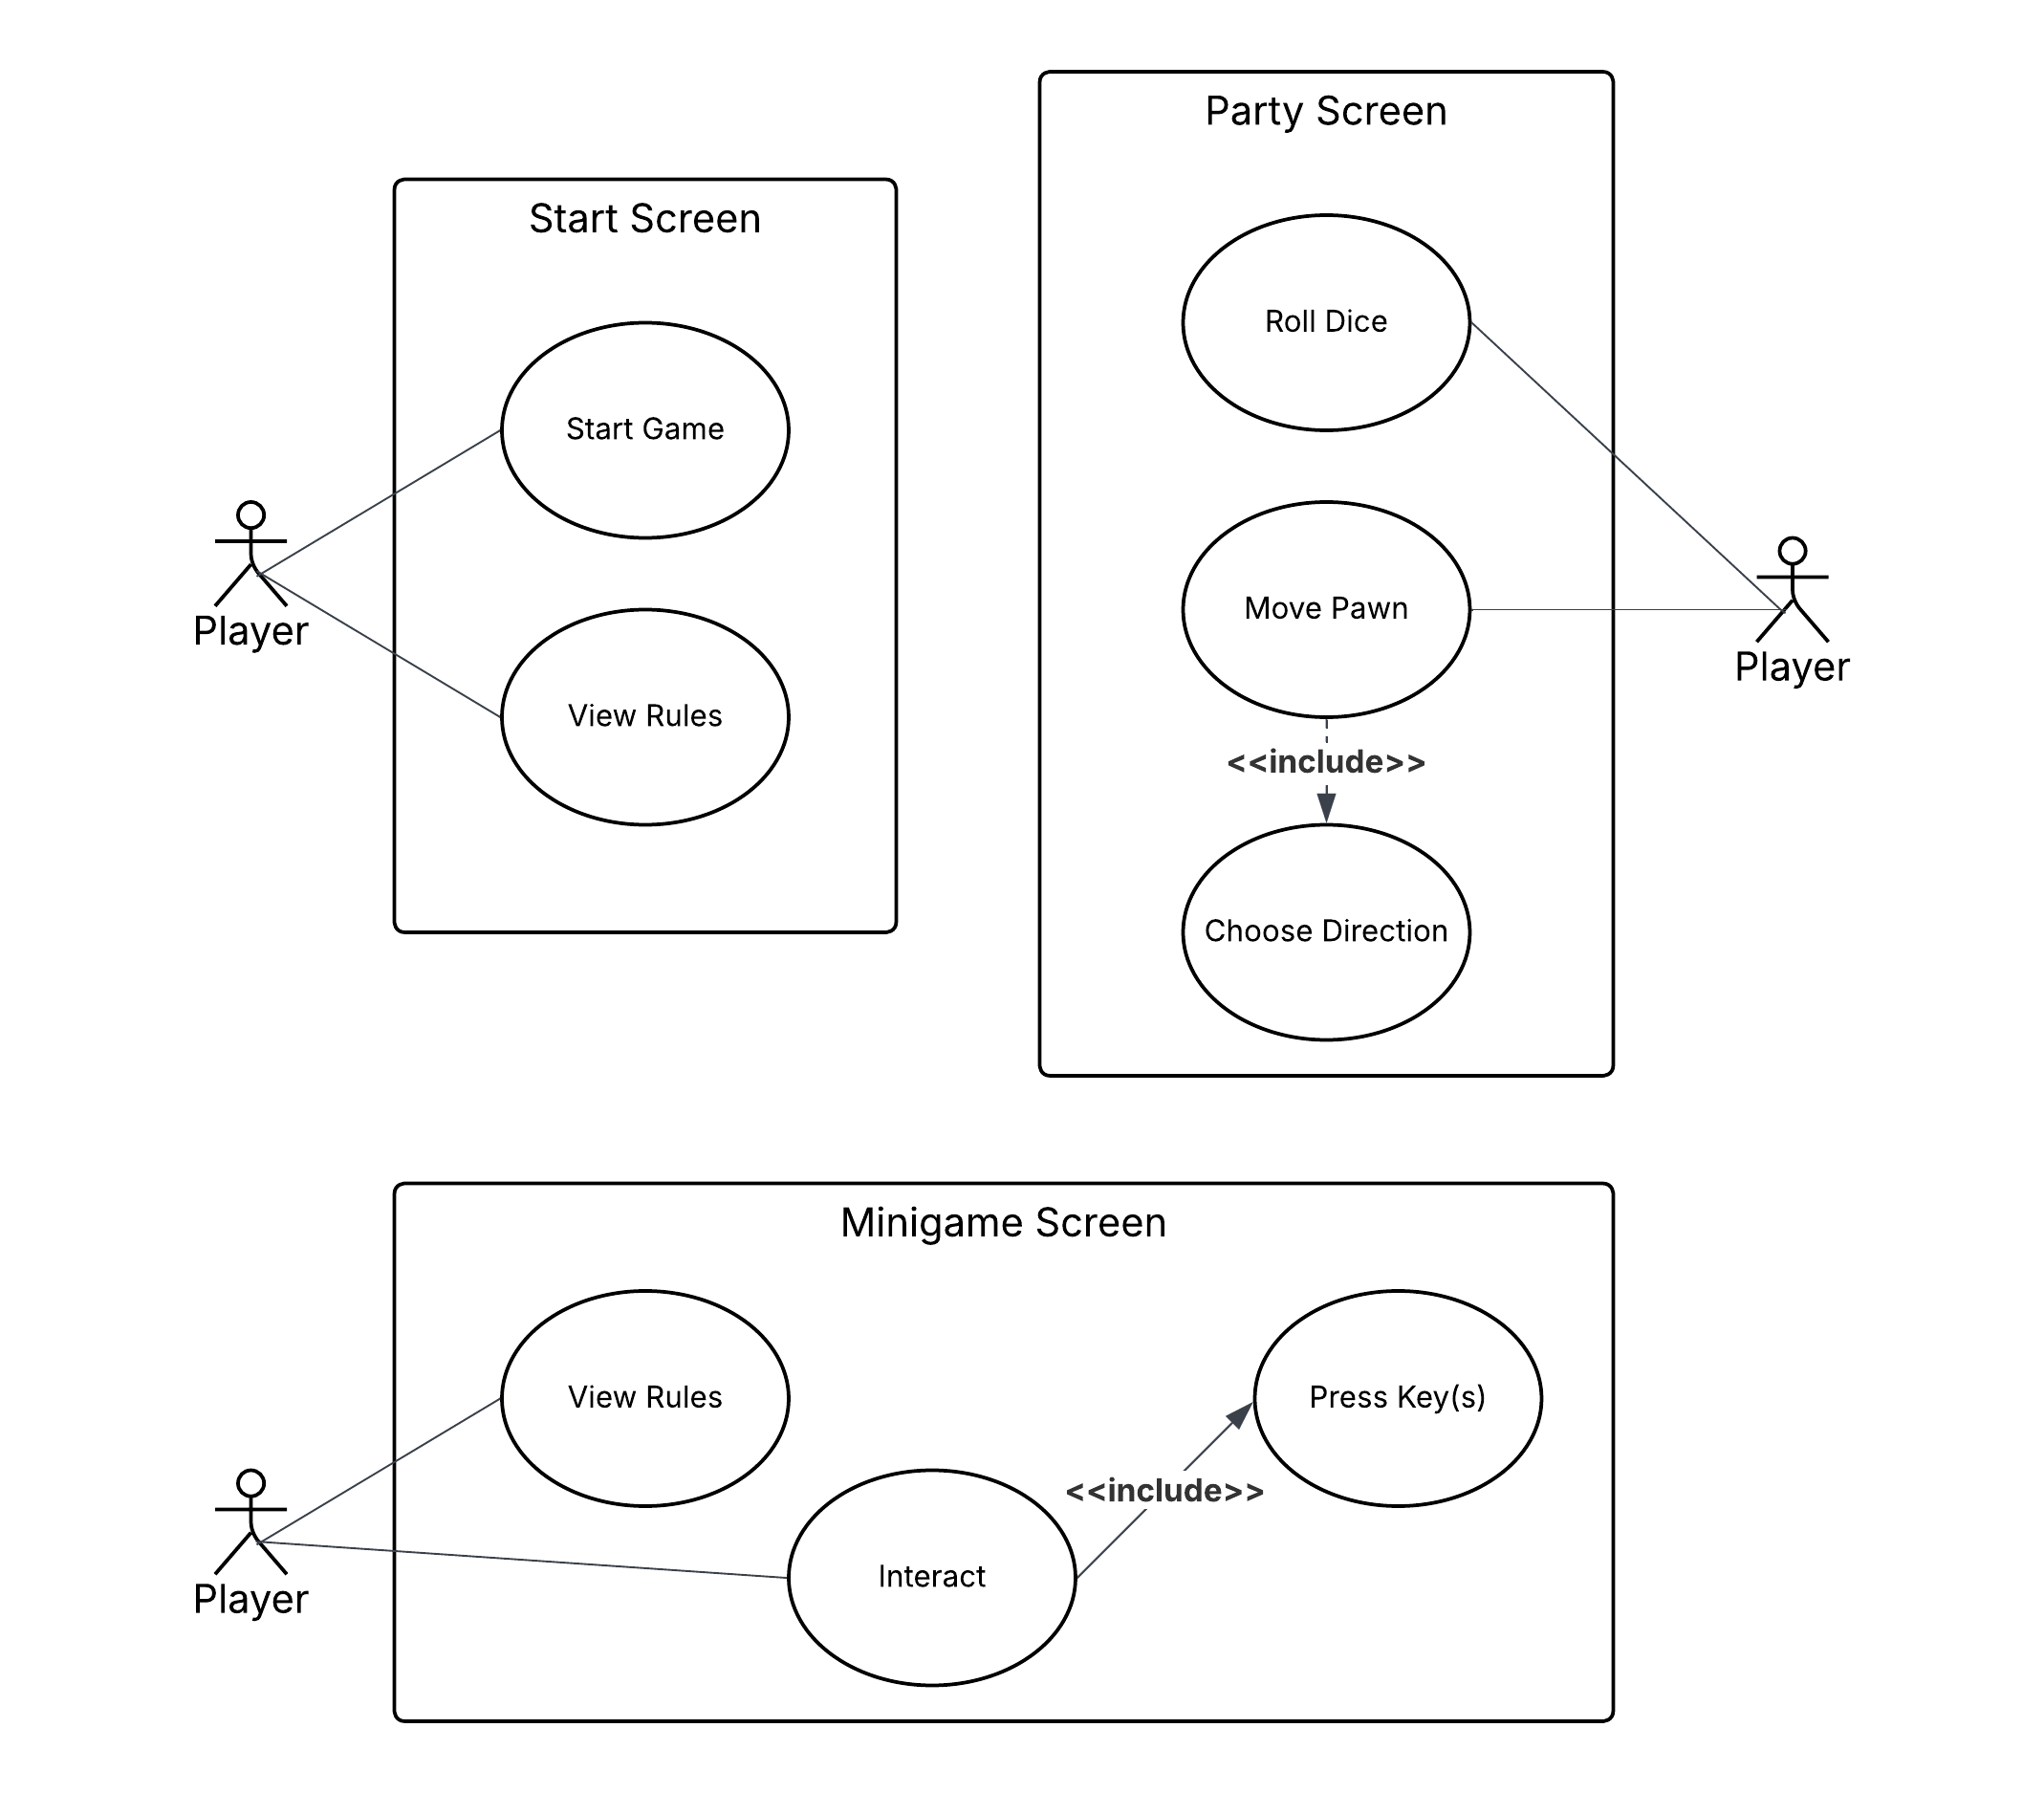
\includegraphics[width=\textwidth]{figures/use-cases.png}
    \caption{Casi d'uso dell'applicazione}
    \label{fig:use-cases}
\end{figure}

\subsubsection{Diagramma degli stati} \label{sec:design-choices:state-diagram}

\subsubsection{Diagramma delle classi} \label{sec:design-choices:class-diagram}
Il diagramma delle classi presentato a figura \ref{fig:class-diagram} è un ampliamento del diagramma presentato precedentemente
(figura \ref{fig:domain-class-diagram}), a cui sono stati aggiunti alcuni dettagli e, soprattutto, le classi di Controller e View.
In particolare la View espone solo il metodo di repaint in quanto il resto delle operazioni, come la gestione degli eventi e dell'input,
viene gestito dal Controller. Quest'ultimo, a sua volta, si occupa di comunicare con il Model per ottenere le informazioni necessareie
e aggiornarne lo stato, che successivamente verrà comunicato alla View. In più sono presenti alcune classi di utility che, nonstante
non siano connesse direttamente ad altre classi, sono riportate per completezza di informazione. Direction e Turn sono due Enum che
rappresentano rispettivamente le direzioni in cui può muoversi una pedina e il turno di gioco e le fasi del gioco. P2d è invece una classe
che rappresenta un punto bidimensionale, utile per rappresentare le coordinate di una pedina o di un oggetto nel tabellone senza 
dover utilizzare una coppia di variabili.
\begin{figure}[ht!]
    \centering
    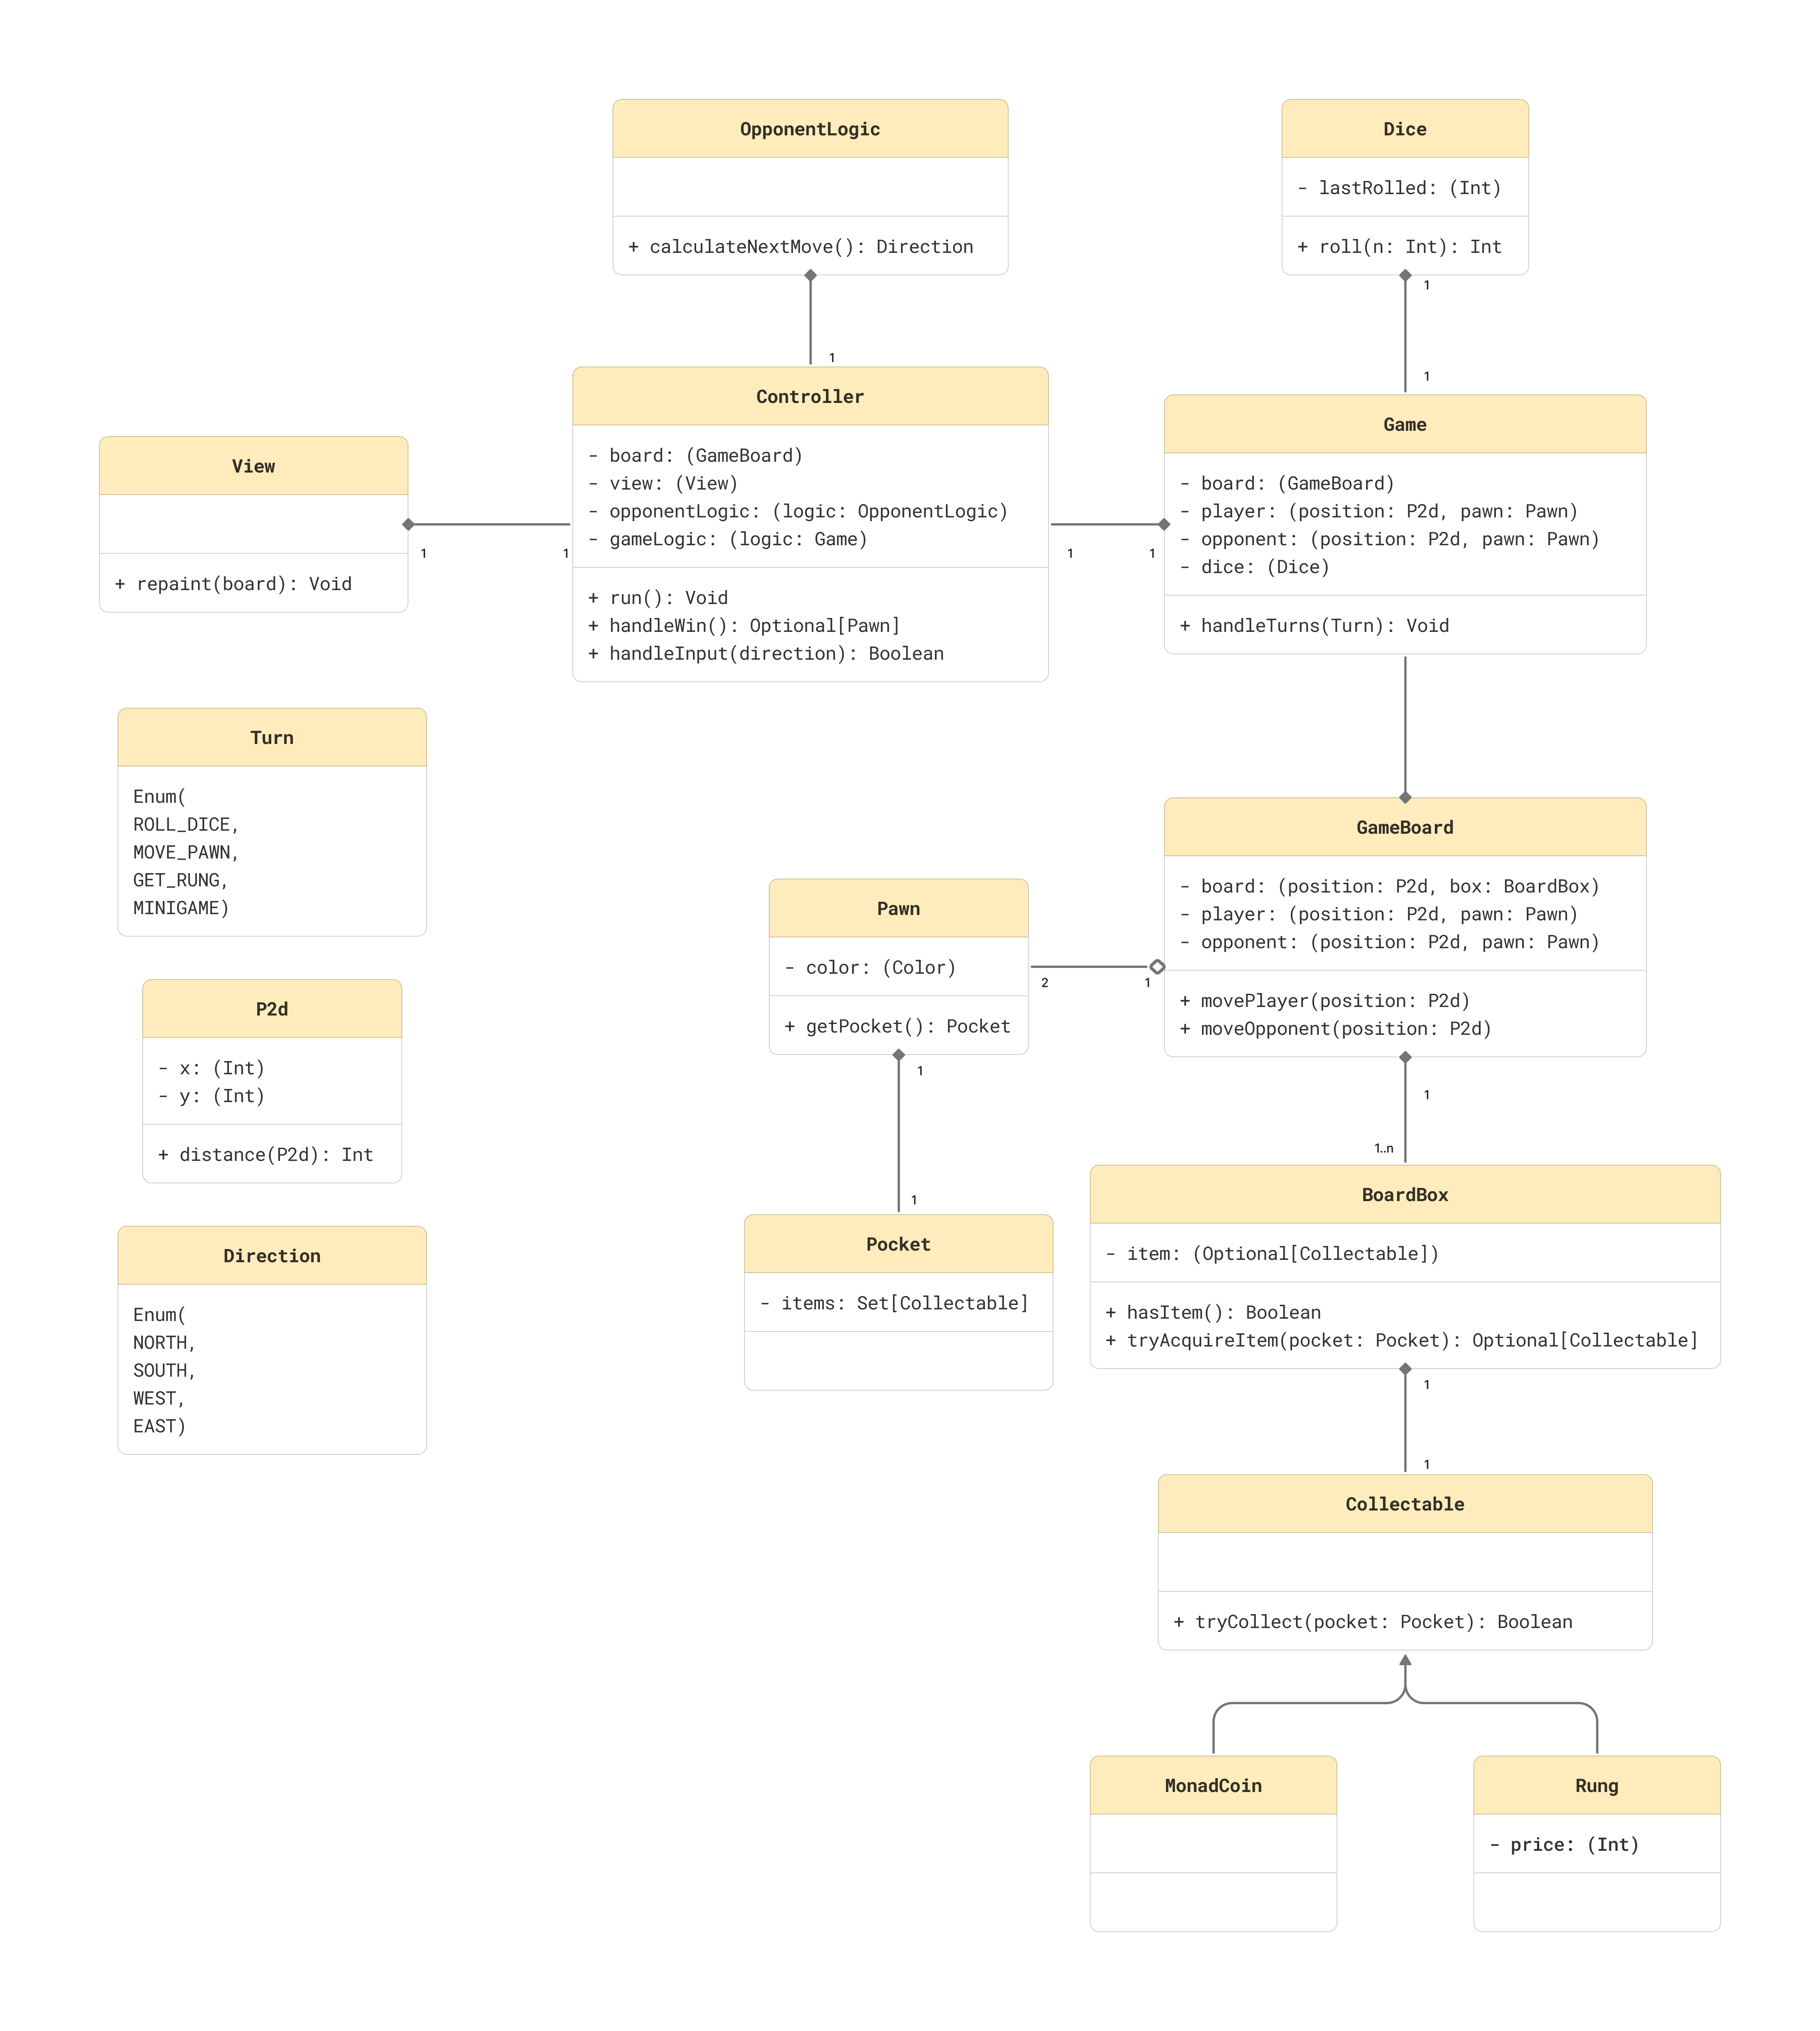
\includegraphics[width=\textwidth]{figures/ClassDiagram_ScalaParty.png}
    \caption{Diagramma delle classi per il tabellone}
    \label{fig:class-diagram}
\end{figure}
